% ============================================================================
%  Bridge Weigh-in-Motion as a regularized Bayesian inverse problem
%  Technical report -- B.Sc. Computational Engineering Science (CES), RWTH Aachen
%
%  COMPILE: upload this folder (report.tex + figures/) to Overleaf and press
%  "Recompile" (pdfLaTeX). Locally: pdflatex report.tex (run twice).
% ============================================================================
\documentclass[11pt,a4paper]{article}

\usepackage[T1]{fontenc}
\usepackage[utf8]{inputenc}
\usepackage{lmodern}
\usepackage[margin=2.3cm]{geometry}
\usepackage{amsmath,amssymb}
\usepackage{graphicx}
\usepackage{booktabs}
\usepackage{siunitx}
\usepackage{caption}
\usepackage{subcaption}
\usepackage[hidelinks]{hyperref}
\usepackage{xcolor}
\usepackage{textcomp}
\usepackage{enumitem}
\newcommand{\EUR}[1]{\texteuro#1}

\sisetup{detect-all}
\graphicspath{{figures/}}
\captionsetup{font=small,labelfont=bf}
\setlist{nosep,leftmargin=1.4em}

% --- RWTH house colours + banner -------------------------------------------
\definecolor{rwthblue}{HTML}{00549F}
\definecolor{rwthblue25}{HTML}{C7DDF2}
\definecolor{rule}{HTML}{8EBAE5}
\newcommand{\rwthbanner}{%
  \noindent\colorbox{rwthblue}{%
    \parbox{\dimexpr\textwidth-2\fboxsep\relax}{%
      \vspace{2.5pt}%
      {\color{white}\textbf{RWTH AACHEN UNIVERSITY}}\hfill
      {\color{white}\footnotesize Computational Engineering Science}%
      \vspace{2.5pt}}}%
  \vspace{1pt}\par\noindent{\color{rule}\rule{\textwidth}{1.3pt}}%
}

\begin{document}

% ---- title block -----------------------------------------------------------
\rwthbanner
\vspace{0.8em}

{\raggedright
  {\LARGE\bfseries Bridge Weigh-in-Motion as a regularized Bayesian inverse problem}\\[0.35em]
  {\large Verification, validation against measured data, and model-error-aware uncertainty}\\[0.8em]
  {\normalsize Muhammet Emir Fil}\\[0.15em]
  {\small B.Sc.\ Computational Engineering Science, RWTH Aachen \quad\textbullet\quad Technical report, \today}\par
}
\vspace{0.6em}
\noindent{\color{rule}\rule{\textwidth}{0.6pt}}
\vspace{1.0em}

% ---- AIM -------------------------------------------------------------------
\noindent\colorbox{rwthblue25}{%
  \parbox{\dimexpr\textwidth-2\fboxsep\relax}{%
  \vspace{3pt}\textbf{Aim.} Build the forward physics of a vehicle crossing a bridge, then run
  it backwards to recover the truck's axle weights (Bridge Weigh-in-Motion), and treat that
  recovery with the discipline an inverse problem needs: analytical verification of every
  forward block, regularization of the ill-posed part, an uncertainty estimate calibrated from
  model error rather than assumed, and validation against real measured bridge data. The goal is
  a B-WIM pipeline in which every number is checked against a reference. The core is
  numpy-only.\vspace{3pt}}}

\vspace{1.0em}

\begin{abstract}
\noindent
A truck crossing a bridge leaves a measurable trace in the structure's response. Read forwards,
that trace predicts the bridge's vibration; read backwards, it recovers the axle weights. The
second reading is Bridge Weigh-in-Motion (B-WIM), an inverse problem that turns an instrumented
bridge into a traffic-speed scale. This report builds the forward physics (an Euler--Bernoulli
beam under a moving, coupled vehicle load), inverts it for the axle loads, and treats the result
the way an inverse problem requires: verification of every forward block against an analytical
reference, regularization of the ill-conditioned tandem-axle split, an uncertainty estimate that
is shown to be badly over-confident on a dynamic bridge and is then re-calibrated from physics,
and validation against real measured data from the KW51 bridge. The core is numpy-only and every
number ships with the reference it was checked against.
\end{abstract}

% ---------------------------------------------------------------------------
\section{Motivation}
% ---------------------------------------------------------------------------
Road and bridge damage grows roughly with the fourth power of axle load (AASHO Road Test): a
truck at twice the legal axle weight does about $16\times$ the structural damage. Static weigh
stations are expensive and easy to evade. B-WIM instead weighs trucks at traffic speed by
inverting the bending response of a bridge that is already instrumented. The same dynamic signal
also carries information about the structure's health (drive-by, vibration-based monitoring). The
engineering questions are therefore those of an inverse problem: how well-posed is the recovery,
how much can a recovered number be trusted, and does the method survive contact with real data.
The rule throughout is that every claim is checked against a reference, and if the code disagrees
with the reference the code is wrong.

% ---------------------------------------------------------------------------
\section{Forward model}
% ---------------------------------------------------------------------------
\paragraph{Bridge.} A simply-supported Euler--Bernoulli beam is discretised with 2-node Hermitian
beam finite elements, two degrees of freedom per node (transverse deflection $w$, rotation
$\theta$). Element consistent mass $\mathbf{M}_e$ and bending stiffness $\mathbf{K}_e$ assemble
into
\begin{equation}
  \mathbf{M}\,\ddot{\mathbf{u}} + \mathbf{C}\,\dot{\mathbf{u}} + \mathbf{K}\,\mathbf{u}
  = \mathbf{F}(t),
  \label{eq:eom}
\end{equation}
with optional Rayleigh damping $\mathbf{C}=\alpha\mathbf{M}+\beta\mathbf{K}$. The reference
structure is a 40\,m highway overpass with $f_1\approx 2.6\,$Hz and $\zeta = 2\,\%$.

\paragraph{Moving load.} A wheel at position $x_p(t)$ in element $e$ is mapped to nodal forces
through the cubic Hermite shape functions $\mathbf{N}(\xi)$,
$\mathbf{F}_e(t) = \mathbf{N}(\xi(x_p,t))^{\top} P(t)$, so $\mathbf{F}(t)$ is rebuilt every step
as the load travels.

\paragraph{Vehicle.} The wheel force is not constant. The truck is a 2-DOF quarter-car (sprung
mass on suspension $k_s,c_s$; unsprung mass on tyre $k_t$) coupled to the beam at the contact
point, so the road profile and the bridge deflection feed back into $P(t)$.

\paragraph{Time integration.} Two integrators are implemented and cross-checked: explicit RK4 on
the state-space form, and implicit Newmark-$\beta$ ($\beta=\tfrac14,\gamma=\tfrac12$,
unconditionally stable). A modal model-order reduction keeping the first $r$ modes provides a
third, cheaper forward path.

\paragraph{Inverse model.} With the section influence line $\mathbf{C}$ assembled from the beam's
response to a unit load at each sampled position, the measured bending-moment history
$\mathbf{m}$ is fit in least squares for the static axle loads $\mathbf{P}$ (Moses' method),
\begin{equation}
  \hat{\mathbf{P}} = (\mathbf{C}^{\top}\mathbf{C})^{-1}\mathbf{C}^{\top}\mathbf{m}.
  \label{eq:moses}
\end{equation}
Equation~\eqref{eq:moses} is extended below to a Tikhonov-regularized and a Bayesian estimator.

\begin{figure}[t]
  \centering
  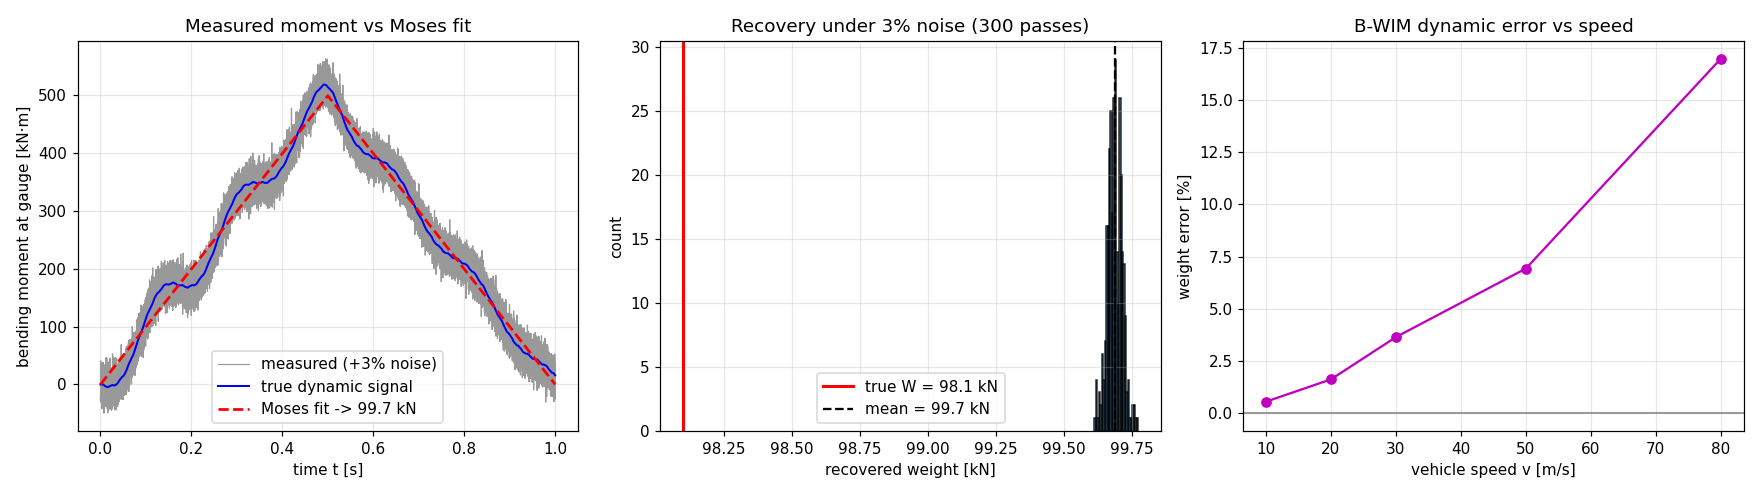
\includegraphics[width=0.8\textwidth]{v4_5_bwim.png}
  \caption{B-WIM round trip. A known truck is driven across the simulated bridge, the bending
  response is measured, and Eq.~\eqref{eq:moses} recovers the axle loads. The recovered gross
  weight tracks the truth to sub-percent in the well-separated-axle case, which is the baseline
  before dynamics and tandem ill-conditioning enter.}
  \label{fig:bwim}
\end{figure}

% ---------------------------------------------------------------------------
\section{Verification: the math is correct}
% ---------------------------------------------------------------------------
Each forward block is checked against an independent analytical reference (Table~\ref{tab:verify}).
These are agreements with closed-form solutions to many significant figures, which is what shows
that the assembly, boundary conditions, and integration are right.

\begin{table}[h]
  \centering
  \caption{Verification of the forward model against analytical references.}
  \label{tab:verify}
  \small
  \begin{tabular}{@{}lll@{}}
    \toprule
    Check & Reference & Result \\
    \midrule
    Static mid-span deflection      & $PL^3/48EI$                       & rel.\ err $\approx 1\times10^{-13}$ \\
    Natural frequencies             & $(n\pi/L)^2\sqrt{EI/\bar m}$       & mode 1 rel.\ err $\approx 4\times10^{-7}$ \\
    Moving constant force           & Frýba closed form                 & peak rel.\ err $\approx 6\times10^{-6}$ \\
    Quarter-car frequencies         & analytic $2\times2$ eigenproblem  & within FFT resolution \\
    Damping $\zeta$                 & free-vibration log-decrement      & within $0.1\,\%$ \\
    Newmark-$\beta$ vs Frýba        & closed-form moving force          & match to $\approx 2\times10^{-4}$ \\
    MOR (3 modes) vs full order     & full-order response               & reproduces to $0.16\,\%$ \\
    \bottomrule
  \end{tabular}
\end{table}

\begin{figure}[h]
  \centering
  \begin{subfigure}{0.32\textwidth}
    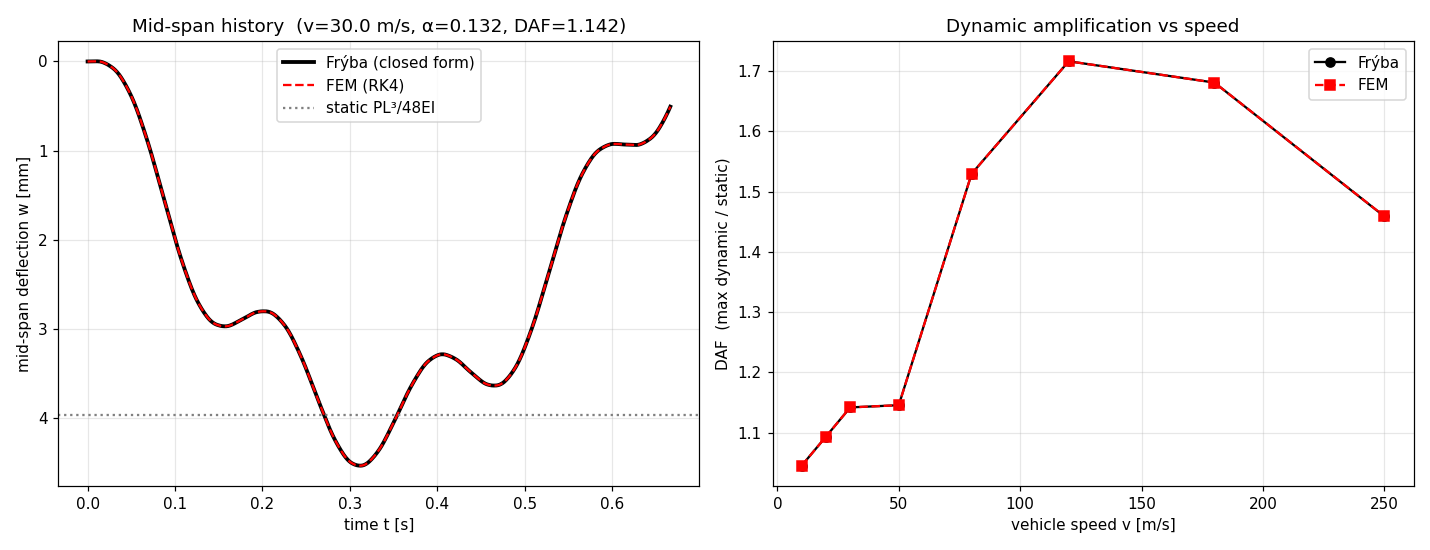
\includegraphics[width=\linewidth]{v2_fryba_check.png}
    \caption{Moving force vs Frýba}
  \end{subfigure}\hfill
  \begin{subfigure}{0.32\textwidth}
    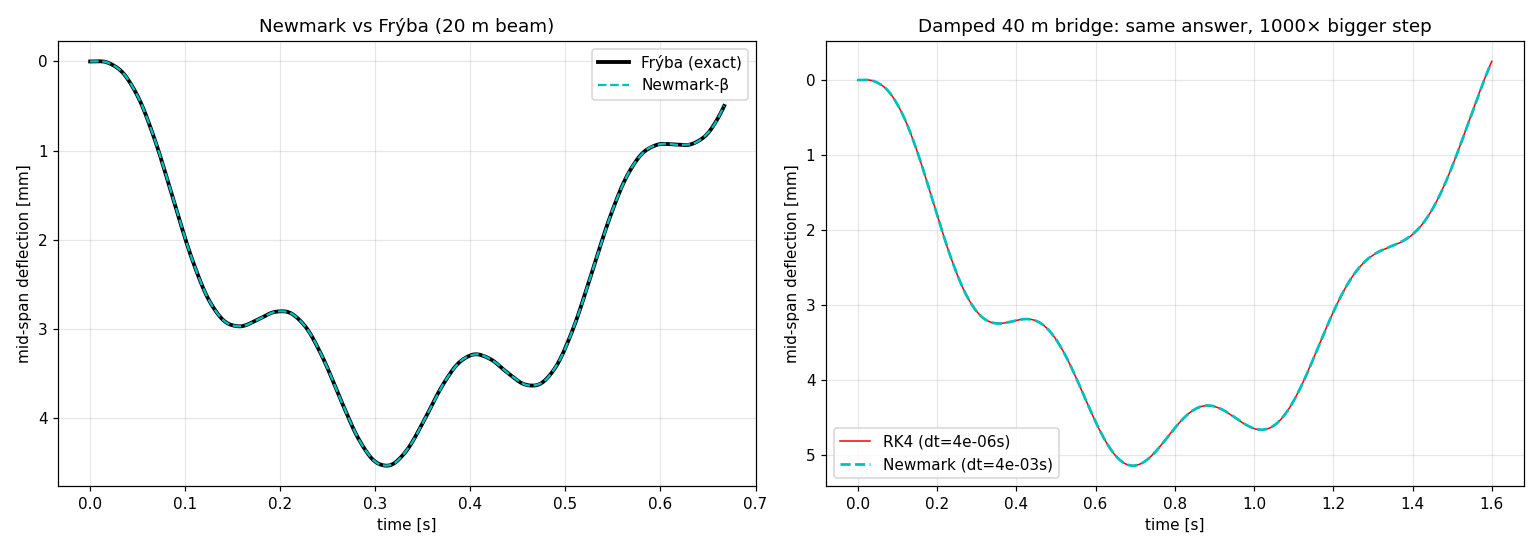
\includegraphics[width=\linewidth]{newmark_verify.png}
    \caption{Newmark-$\beta$ vs closed form}
  \end{subfigure}\hfill
  \begin{subfigure}{0.32\textwidth}
    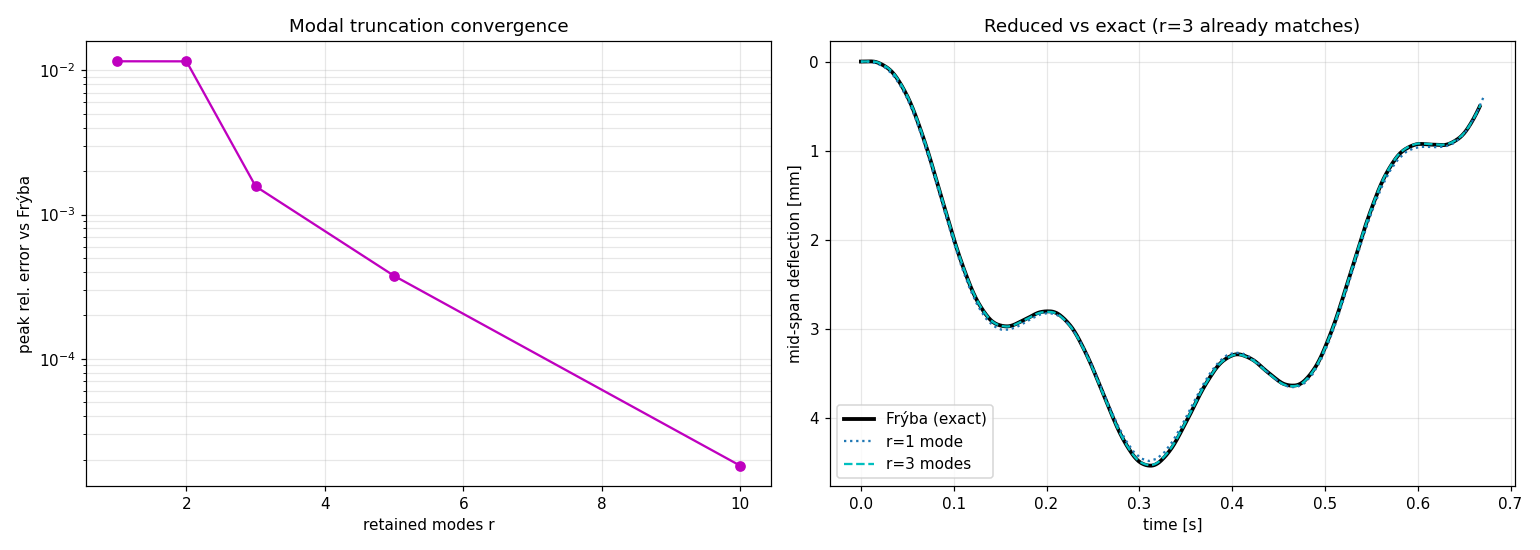
\includegraphics[width=\linewidth]{mor_verify.png}
    \caption{3-mode MOR vs full order}
  \end{subfigure}
  \caption{Representative verification figures. The FEM mid-span deflection (markers) lies on the
  analytical curve (line) in each case, and the implicit and reduced-order integrators reproduce
  the explicit full-order response.}
  \label{fig:verify}
\end{figure}

% ---------------------------------------------------------------------------
\section{Validation and uncertainty: the model means something}
% ---------------------------------------------------------------------------
Verification is not validation. The four results below separate ``the math is right'' from ``the
answer is trustworthy''.

\subsection{Model-error-aware uncertainty}
Casting Eq.~\eqref{eq:moses} as a linear-Gaussian inverse problem gives a posterior over the
weight: the mean is the Moses point estimate, the covariance is
$\sigma^2(\mathbf{C}^{\top}\mathbf{C})^{-1}$ with $\sigma$ from the fit residual, and from these
follow a 95\,\% credible interval and a probability of exceeding the legal limit.

A self-consistent coverage test, in which the synthetic data and the inverse both use the static
influence line, returns 95.3\,\% coverage (Fig.~\ref{fig:coverage}, right). This is reassuring but
only verifies the linear-Gaussian machinery; it is circular. The honest test replaces the forward
model with the full coupled dynamic FEM. The recovered weight is then biased by dynamic
amplification (about $+0.3\,\%$ quasi-static, rising to $+5\,\%$ at 40\,m/s), and because the
residual $\sigma$ measures goodness of fit (the signal still looks influence-line-shaped) rather
than the dynamic scale error, the nominal 95\,\% interval's true coverage collapses to nearly
zero. The fix is physical rather than fitted: the RMS dynamic bias over the highway speed band,
about $3.1\,\%$, is the model-error term that restores calibration. Inflating the posterior by
this physics-derived term returns the coverage to nominal, so the uncertainty is calibrated from
the dynamics it was missing.

\begin{figure}[h]
  \centering
  \begin{subfigure}{0.48\textwidth}
    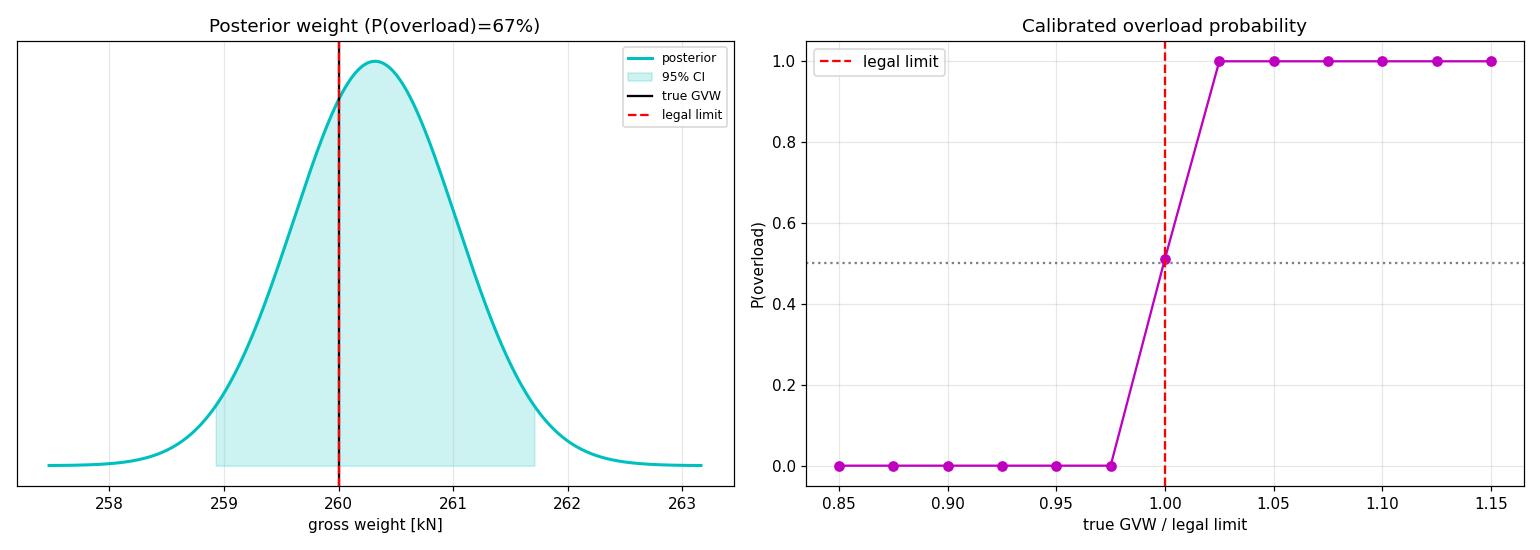
\includegraphics[width=\linewidth]{bayesian_bwim.png}
    \caption{Bayesian posterior with 95\,\% credible interval and $P(\text{overload})$.}
  \end{subfigure}\hfill
  \begin{subfigure}{0.48\textwidth}
    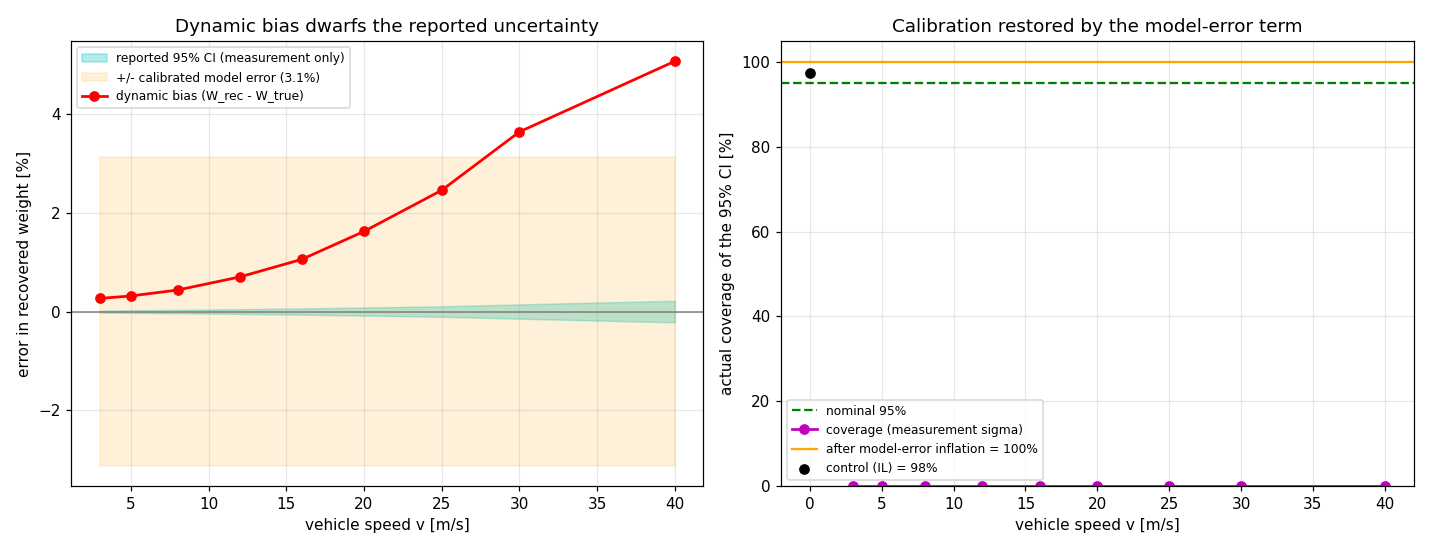
\includegraphics[width=\linewidth]{coverage_modelerror.png}
    \caption{Self-consistent 95.3\,\% coverage collapses under the dynamic forward model; a
    3.1\,\% physics-derived term restores it.}
  \end{subfigure}
  \caption{Model-error-aware uncertainty. The result is the gap between the circular test and the
  honest one, and that the gap closes with a number derived from the physics rather than tuned.}
  \label{fig:coverage}
\end{figure}

\subsection{Regularizing the ill-posed axle split}
Moses' method recovers gross weight to better than 1\,\% but splits closely spaced (tandem) axles
poorly. The cause is linear-algebraic: a tandem makes two columns of $\mathbf{C}$ nearly parallel,
so $\operatorname{cond}(\mathbf{C}^{\top}\mathbf{C})$ rises from about 9 at 8\,m spacing to about
2000 at 0.5\,m, and the split amplifies noise. Tikhonov regularization,
\begin{equation}
  \hat{\mathbf{P}}_\lambda
  = (\mathbf{C}^{\top}\mathbf{C} + \lambda^2 \mathbf{I})^{-1}\mathbf{C}^{\top}\mathbf{m},
\end{equation}
with $\lambda$ chosen at the L-curve corner ($\lambda^\star\approx 7.9$), cuts the per-axle scatter
by about $6\times$ (from 16\,\% to 2.6\,\%) for a small bias, while leaving the well-posed gross
weight unchanged (Fig.~\ref{fig:reg}). This is the bias--variance trade-off of an ill-posed
inverse, made explicit and controlled.

\begin{figure}[h]
  \centering
  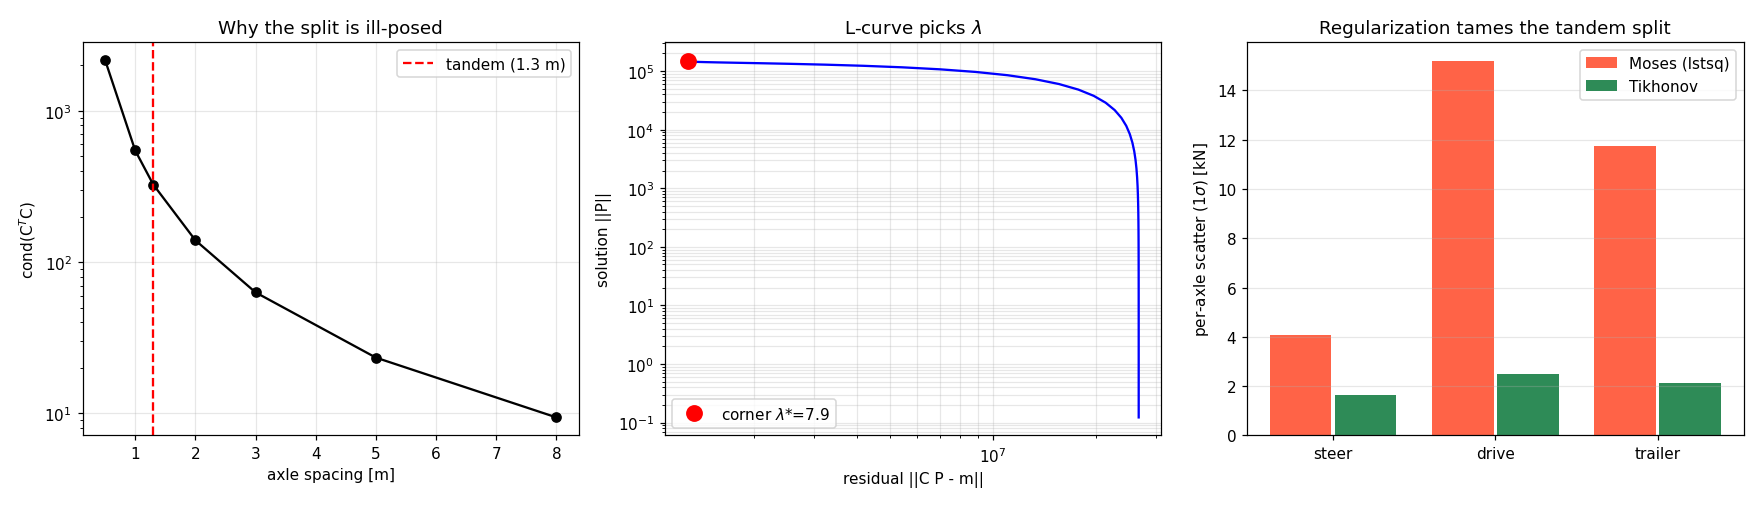
\includegraphics[width=0.95\textwidth]{regularize.png}
  \caption{Ill-conditioning and its cure. Left: $\operatorname{cond}(\mathbf{C}^{\top}\mathbf{C})$
  versus axle spacing. Middle: the L-curve corner selects $\lambda^\star$. Right: regularization
  cuts the tandem-split scatter by about $6\times$ while the gross weight is untouched.}
  \label{fig:reg}
\end{figure}

\subsection{Validation against real data (KW51)}
The 16-month tracked-modal-frequency record of the instrumented KW51 railway bridge (Leuven; public
Zenodo dataset) is ground truth no model can argue with. It confirms the drive-by-SHM premise: a
real, dated retrofit (stiffening) shifts the modal frequencies by up to $+2.6\,\%$. It also exposes
the dominant confounder: temperature swings the same frequencies by a comparable amount (up to
about $3.8\,\%$), and for some modes the temperature swing exceeds the retrofit jump. Removing the
temperature trend (fit on the healthy period) sharpens the change from a raw to a
temperature-corrected residual, for example from $9.8\,\sigma$ to $17.3\,\sigma$ for one mode. This
is the limit the synthetic damage study predicted, now confirmed in the field: a single global
frequency is a blunt, environment-contaminated indicator that detects but cannot localize.

\begin{figure}[h]
  \centering
  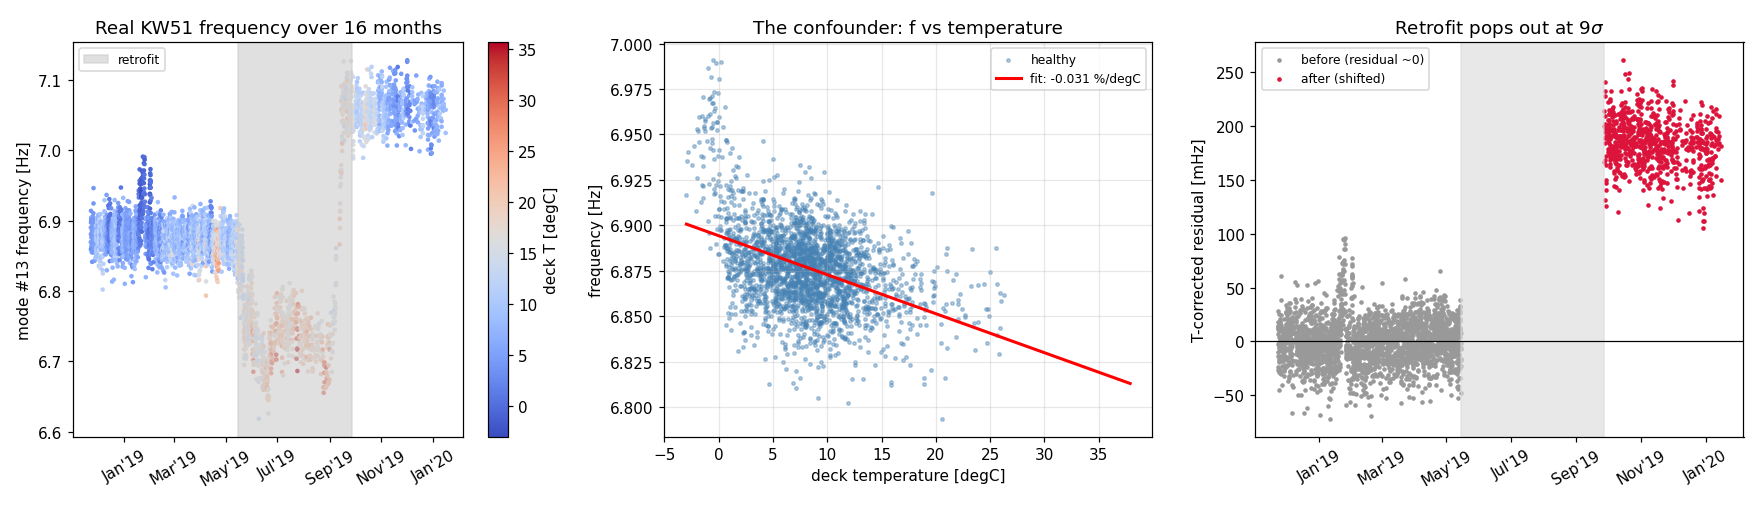
\includegraphics[width=0.9\textwidth]{kw51_validation.png}
  \caption{Validation on real KW51 data. The retrofit step is visible in the tracked modal
  frequencies, but temperature contaminates the signal at a comparable amplitude; a temperature
  correction is required before a stiffness change is detectable.}
  \label{fig:kw51}
\end{figure}

\subsection{From weight to decision (fatigue economics)}
A recovered weight is only useful if it drives a decision. Steel-detail fatigue follows an S--N law
with slope $m$ (Eurocode EN 1993-1-9, $m=3$; AASHTO pavement, $m=4$), so damage per pass scales as
$(W/W_\text{ref})^m$: a $2\times$ overload does $8$ to $16\times$ the damage. Over a simulated
traffic stream the damage concentrates sharply, with the heaviest 10\,\% of trucks causing about
45\,\% of the fatigue damage and the overloaded minority about half, and B-WIM identifies exactly
those trucks. An asset-depreciation estimate puts one heavy crossing at about \EUR{}10 of bridge
life against \EUR{}0.80 for a legal pass, which is the quantified case for self-funding overload
enforcement.

\begin{figure}[h]
  \centering
  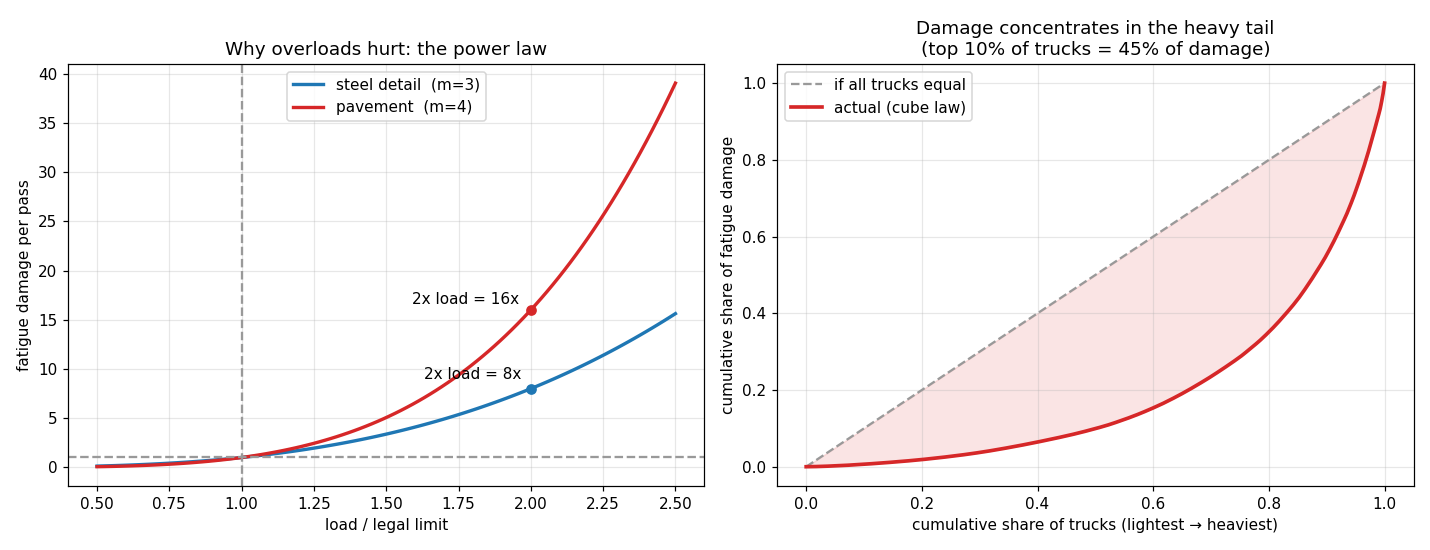
\includegraphics[width=0.9\textwidth]{fatigue_economics.png}
  \caption{From a recovered weight to a decision. The fourth-power law concentrates fatigue damage
  in a few heavy trucks (Pareto), which B-WIM is the tool to catch.}
  \label{fig:fatigue}
\end{figure}

% ---------------------------------------------------------------------------
\section{Limitations}
% ---------------------------------------------------------------------------
\begin{itemize}
  \item One simply-supported single span; linear, small-displacement Euler--Bernoulli theory.
  \item A single quarter-car (one wheel path); the multi-axle B-WIM uses constant axle forces.
  \item The drive-by study detects a global stiffness change but does not localize it, since a
        single fundamental frequency cannot by construction.
  \item KW51 is a 115\,m steel bowstring arch, not a simply-supported beam, so it validates the
        SHM behaviour and method rather than the FEM geometry.
  \item B-WIM here uses the analytical influence line; field systems calibrate it from a known
        truck and lose accuracy to road roughness, multiple vehicles, and temperature.
\end{itemize}

% ---------------------------------------------------------------------------
\section{Reproducibility}
% ---------------------------------------------------------------------------
\begin{sloppypar}
The solver is numpy-only. Each result is produced by a \texttt{verify\_*.py} script that prints the
numbers and saves the figure shown here: \texttt{verify\_v2.py} for Frýba, \texttt{verify\_newmark.py},
\texttt{verify\_mor.py}, \texttt{verify\_coverage.py}, \texttt{verify\_regularize.py},
\texttt{verify\_kw51.py}, and \texttt{verify\_fatigue.py}. An interactive web demo animates the
crossing and the live weighing.
\end{sloppypar}

% ---------------------------------------------------------------------------
\begin{thebibliography}{9}
\small
\bibitem{aasho} AASHO Road Test (1962); fourth-power load-equivalency law (80\,kN ESAL).
\bibitem{fryba} L.\ Frýba, \emph{Vibration of Solids and Structures under Moving Loads},
  Noordhoff, 1972.
\bibitem{moses} F.\ Moses, ``Weigh-in-motion system using instrumented bridges,''
  \emph{J.\ Transp.\ Eng.}, 105(3), 1979.
\bibitem{obrien} E.\ OBrien et al., ``A regularised solution to the bridge weigh-in-motion
  equations,'' \emph{Int.\ J.\ Heavy Vehicle Systems}, 2009.
\bibitem{hansen} P.\,C.\ Hansen, ``The L-curve and its use in the numerical treatment of inverse
  problems,'' 1999.
\bibitem{kw51} K.\ Maes \& G.\ Lombaert, ``Monitoring data for railway bridge KW51,''
  Zenodo 3745914 (2020).
\bibitem{cost323} COST 323, \emph{European Specification on Weigh-in-Motion of Road Vehicles}.
\bibitem{ec3} Eurocode EN 1993-1-9, \emph{Fatigue strength of steel structures}.
\end{thebibliography}

\end{document}
